\section{Controlling the Virtual Rover NEW}
\label{sec:control_vr_model}

\begin{figure}[!h]
	\centering
	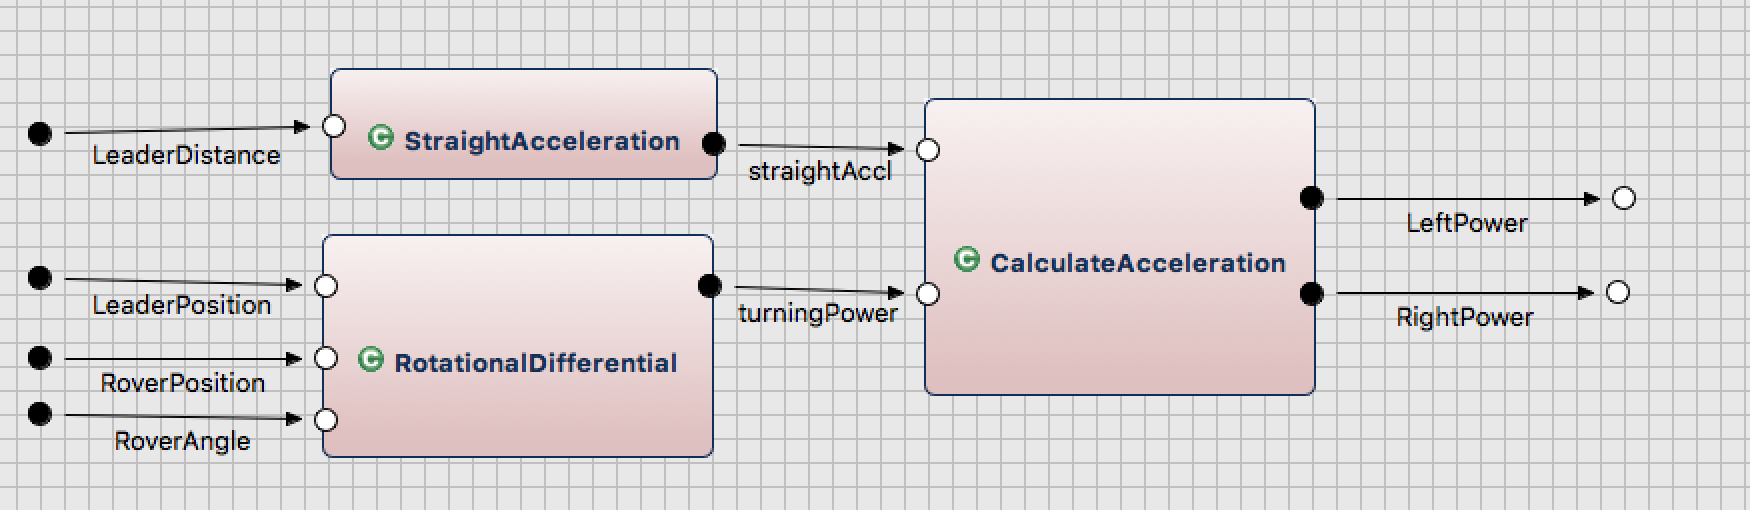
\includegraphics[width=1\textwidth]{images/acc.png}
	\caption{The controller for the Virtual Rover}
	\label{fig:acc}
\end{figure}

In \fig\ref{fig:acc} we depict the top-level model of the controller for the
follower vehicle. The controller is meant to operate in a loop by reading the
 {distance} to
the leader rover, the GPS coordinates of the leader (\textit{LeaderPosition}) and the rover's own (\textit{RoverPosition}) GPS
coordinates, and the followers orientation with respect to north (\textit{RoverAngle}).
Note that the inputs to the model appear in \fig\ref{fig:acc}  as small
black circles, while the outputs have the same shape but are white. By the
input values the controller constantly updates the power provided to the
wheels.

The controller for the virtual rover is composed by three \af components,
as follows:
\subsection{Component StraightPower}
The \textsf{StraightPower} component is responsible for calculating the required forward power based on the distance with the leader.

This component is composed of two components as shown in \fig\ref{fig:straight}. The component \textit{CalculateDistanceError} calculates the \textit{error} with respect to the ideal distance with the leader. For this challenge problem the follower was required to remain in the distance range between 12 and 15 from the leader. So we have taken the ideal distance as the average of these two values, i.e., 13.5. This is a constant and can be changed for easily for a different range.

\begin{figure}[!h]
	\centering
	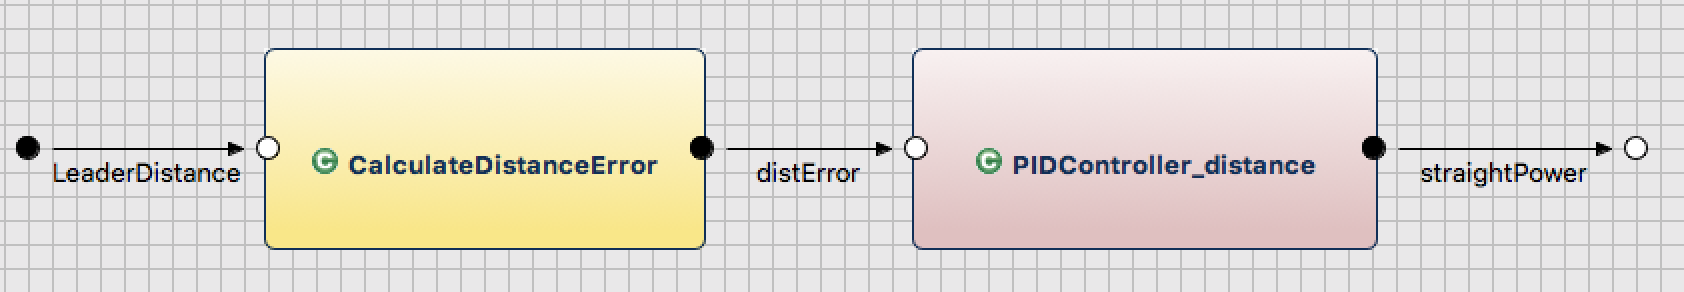
\includegraphics[width=1\textwidth]{images/straight.png}
	\caption{Component for calculating required forward power.}
	\label{fig:straight}
\end{figure}


We then use this \textit{error} and feed it to a PID controller for calculating the forward power. The general equation for a PID controller is:
\begin{equation}
u = K_Pe + K_II + K_DD
\label{formula:pidController}
\end{equation}

For calculating the forward power we have used the following constant values: $K_P = 5$, $K_I=1.5$, $K_D=30$.


\subsection{Component RotationalDifferential}

The rover turns when the left and right wheels rotate at different speeds. The magnitude of the difference is proportional to the turning angle. When the leader turns the follower also has to turn in order to follow the leader. 

The \textsf{RotationalDifferential} component calculates the required difference between the power applied to the right and the left wheel to turn the rover such that it follows the leader.

The component \textsf{bearingAngle} calculates the bearing of the leader with respect to north when seen from follower. This calculation uses the GPS positions of the follower and the leader. We then calculate he \textit{angleError} i.e., the difference between the orientation of the follower (with respect to north) and the bearing angle. We then feed this \textit{angleError} in another PID controller to give us the required difference in powers. The sign of this value decides the direction of the turning.

\begin{figure}[!h]
	\centering
	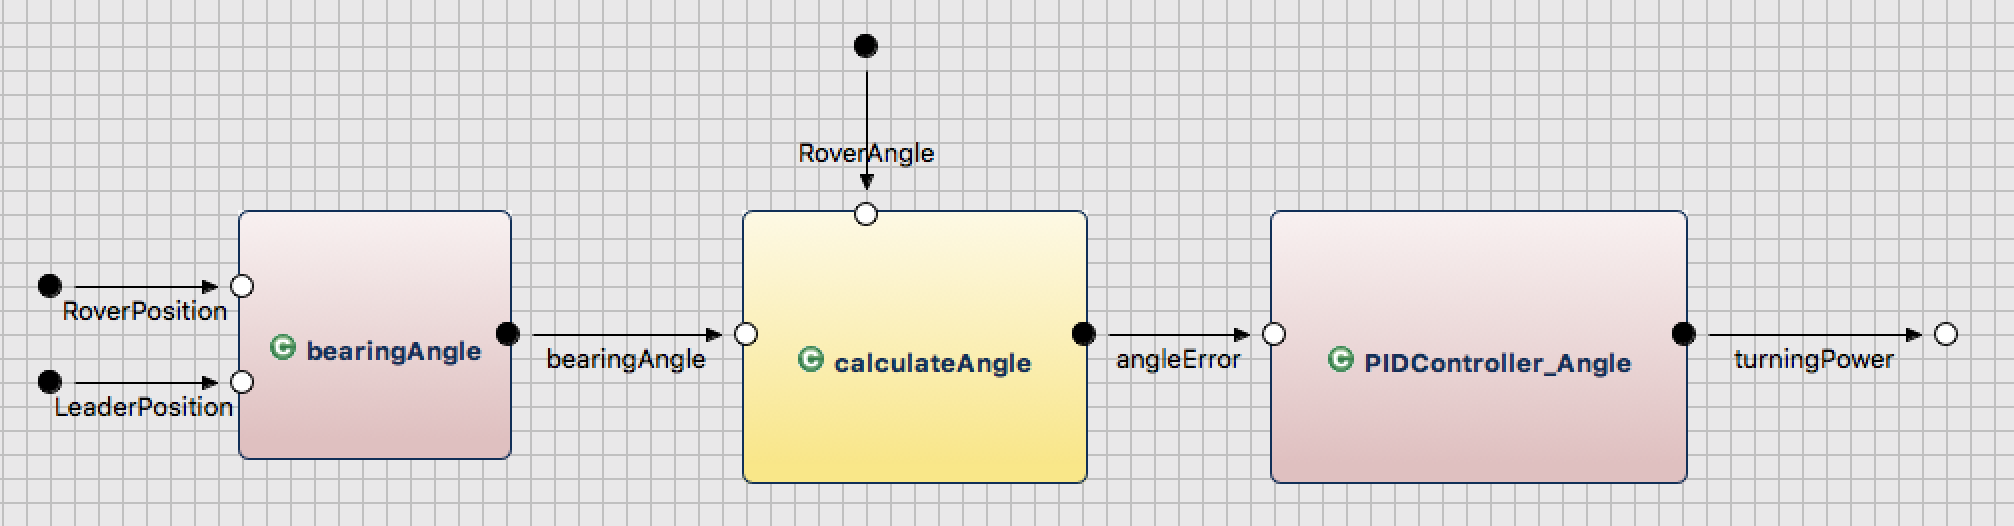
\includegraphics[width=1\textwidth]{images/rotation.png}
	\caption{Component for calculating the differential power.}
	\label{fig:rotation}
\end{figure}

The constants used of the PID controller (equation \ref{formula:pidController})for calculating rotational differential are: $K_P = 2$, $K_I=0.75$, $K_D=10$.

\subsection{Component CalculateFinalPower}
The \textsf{CalculateFinalPower} component takes the forward power and differential, and outputs the final power to apply to the right and left wheels. In addition to calculating the values for the right and left power it also normalizes the power in case the calculated value exceeds the maximum.

The setup of the rover challenge also provides the percentage of time during which the rover was in the expected distance limits. At present the system developed is staying in these limits consistently over 70\%. This is a matter of tuning the values of the PID controller.